%                      Code_Saturne version 1.3
%                      ------------------------
%
%     This file is part of the Code_Saturne Kernel, element of the
%     Code_Saturne CFD tool.
%
%     Copyright (C) 1998-2007 EDF S.A., France
%
%     contact: saturne-support@edf.fr
%
%     The Code_Saturne Kernel is free software; you can redistribute it
%     and/or modify it under the terms of the GNU General Public License
%     as published by the Free Software Foundation; either version 2 of
%     the License, or (at your option) any later version.
%
%     The Code_Saturne Kernel is distributed in the hope that it will be
%     useful, but WITHOUT ANY WARRANTY; without even the implied warranty
%     of MERCHANTABILITY or FITNESS FOR A PARTICULAR PURPOSE.  See the
%     GNU General Public License for more details.
%
%     You should have received a copy of the GNU General Public License
%     along with the Code_Saturne Kernel; if not, write to the
%     Free Software Foundation, Inc.,
%     51 Franklin St, Fifth Floor,
%     Boston, MA  02110-1301  USA
%
%-----------------------------------------------------------------------
%
\programme{bilsc2}

\vspace{1cm}
%%%%%%%%%%%%%%%%%%%%%%%%%%%%%%%%%%
%%%%%%%%%%%%%%%%%%%%%%%%%%%%%%%%%%
\section{Fonction}
%%%%%%%%%%%%%%%%%%%%%%%%%%%%%%%%%%
%%%%%%%%%%%%%%%%%%%%%%%%%%%%%%%%%%

  Dans ce sous-programme, appel\'e par \fort{codits} et \fort{turbke}, sont calcul\'ees les contributions au bilan explicite des termes
convectifs et diffusifs reconstruits
(sur maillages non orthogonaux et si l'utilisateur le d\'esire) du second membre
d'une \'equation de convection/diffusion pour un scalaire $a$. Ces termes s'\'ecrivent de
facon g\'en\'erique \footnote{Ils interviennent notamment dans le second
membre du syst\`eme en incr\'ements pour la cellule $I$ de l'\'etape de pr\'ediction des vitesses : $\mathcal{EM}(\delta\vect{u}^{k+1},I) =
\mathcal{E}(\vect{u}^{n+1/2,k},I)$  ({\it cf}. \fort{navsto} pour plus de d\'etails).}:

\begin{equation}\label{Base_Bilsc2_eq_continue}
\begin{array}{ll}
\mathcal{B_{\mathcal{\beta}}}((\rho\,\vect{u})^{n},a)
&=\underbrace{-\dive(\,(\rho \vect{u})^{n}a)}_{\text {partie convective}}
+\underbrace{\dive(\,\beta\,\grad a)}_{\text{partie diffusive}}\\
\end{array}
\end{equation}

avec $\rho$, $\vect{u}$, $\beta$ et $a$ variables connues \`a l'instant ${t^n}$.

%%%%%%%%%%%%%%%%%%%%%%%%%%%%%%%%%%
%%%%%%%%%%%%%%%%%%%%%%%%%%%%%%%%%%
\section{Discr\'etisation}
%%%%%%%%%%%%%%%%%%%%%%%%%%%%%%%%%%
%%%%%%%%%%%%%%%%%%%%%%%%%%%%%%%%%%
\subsection{\bf Partie convective}
En s'inspirant des notations adopt\'ees dans le sous-programme \fort{navsto}, le  bilan explicite correspondant \`a l'int\'egration sur une cellule $\Omega_i$
de la partie convective $-{\dive(\,(\rho\,\vect{u})^n  a)}$ de $\mathcal{B_{\mathcal{\beta}}}$
 peut s'\'ecrire sous forme
d'une somme de flux num\'eriques $F_{\,ij}$ calcul\'es aux faces des
cellules purement internes et de flux num\'eriques $F_{\,b_{ik}}$
calcul\'es aux faces de bord du domaine $\Omega$.
Soient $Vois(i)$ l'ensemble des centres des cellules voisines de ${\Omega_i}$ et
$\gamma_b(i)$ l'ensemble des centres des faces de bord de ${\Omega_i}$, s'ils existent. On a donc~:

\begin{equation}\notag
\int_{\Omega_i}{\dive( (\rho \vect{u})^n  a )\, d\Omega} =
\sum_{j\in Vois(i)}{F_{\,ij}((\rho \vect{u})^n, a)}
+\sum_{k\in {\gamma_b(i)}} {F_{\,{b}_{ik}}((\rho \vect{u})^n,a)}
\end{equation}

en posant :
\begin{equation}
F_{\,ij}((\rho \vect{u})^n,a) = \left[{(\rho \vect{u})_{\,ij}^n} \text{.}\, \vect{S}_{\,ij}\right]\ a_{\,f,ij}
\end{equation}

\begin{equation}
F_{\,{b}_{ik}}((\rho \vect{u})^n, a) =  \left[{(\rho \vect{u})_{\,{b}_{ik}}^n} \text{.}\, \vect{S}_{\,{b}_{ik}}\right]\ {a_f}_{\,{b}_{ik}}
\end{equation}
o\`u $a_{\,f,ij}$ et ${a_f}_{\,{b}_{ik}}$ repr\'esentent les valeurs aux faces
internes et de bord respectivement.\\

On rappelle~:\\
\begin{figure}[h]
\hspace*{1cm}\parbox{8cm}{%
\centerline{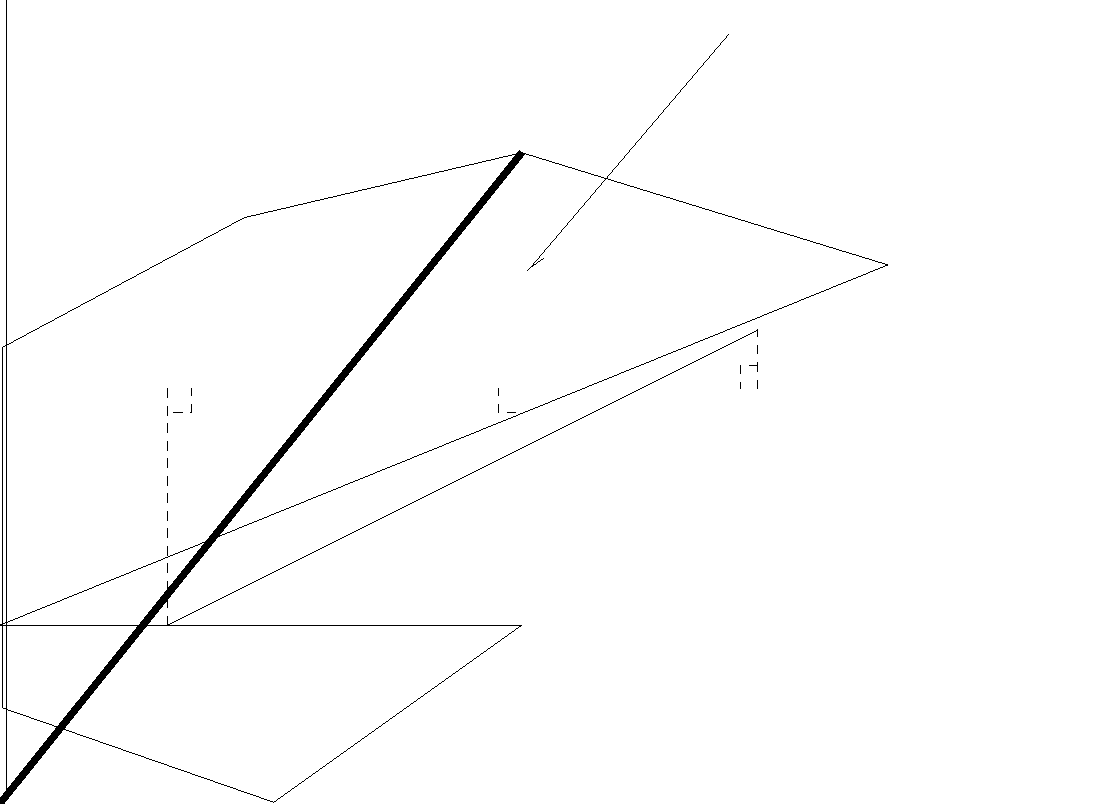
\includegraphics[height=4cm]{../Base/Bilsc2/Images/facette.pdf}}}
\parbox{8cm}{%
\centerline{
\includegraphics[height=4cm]{../Base/Bilsc2/Images/facebord.pdf}}}
\caption{\label{Base_Bilsc2_fig_geom}D\'efinition des diff\'erentes entit\'es
g\'eom\'etriques pour les faces internes (gauche) et de bord (droite).}
\end{figure}
\begin{equation}\notag
\displaystyle\alpha_{ij}=\frac{\overline{FJ'}}{\overline{I'J'}} \text{\ d\'efini aux faces internes uniquement et}
\end{equation}
\begin{equation}\notag
\vect{u}_{K'} = \vect{u}_{K}+(\ggrad{\vect{u}})_K\text{.}\, \vect{KK'}\, \text{\
\`a l'ordre 1 en espace, pour ${K = I \,\text{ou}\, J}$}
\end{equation}\\
La valeur du flux convectif ${F_{\,ij}}$  d\'epend du type de sch\'ema num\'erique choisi. Il en existe trois dans ce sous-programme :


\renewcommand{\arraystretch}{2.}
\begin{tabular}{ll}
\multicolumn{2}{l}{$\bullet\ $un sch\'ema d\'ecentr\'e amont d'ordre 1 (upwind)~:}\\
&$F_{\,ij}((\rho \vect{u})^n,a)=
F^{\it{ amont}}_{\,ij}((\rho \vect{u})^n,a)$\\
o\`u :&
$a_{\,f,ij}= \left\lbrace\begin{array}{l}
a_I \text{ si }(\rho \vect{u})_{\,ij}^n\,.\,\vect{S}_{\,ij}\geqslant 0\\
a_J \text{ si }(\rho \vect{u})_{\,ij}^n\,.\,\vect{S}_{\,ij} < 0
\end{array}\right.$\\

\multicolumn{2}{l}{$\bullet\ $un sch\'ema centr\'e pur~:}\\
&$F_{\,ij}((\rho \vect{u})^n,a)=
F^{\text{\it{ centr\'e}}}_{\,ij}((\rho \vect{u})^n,a)$\\
avec :&$a_{\,f,ij}= \alpha_{ij} a_{I'}+(1-\alpha_{ij}) a_{J'}$\\
\multicolumn{2}{l}{$\bullet\ $un sch\'ema d\'ecentr\'e amont d'ordre 2, SOLU \footnotemark (Second Order Linear Upwind)~:}\\
&$F_{\,ij}((\rho \vect{u})^n,a)=
F^{\text{\it { SOLU}}}_{\,ij}((\rho \vect{u})^n,a)$ \\
avec :&
$a_{\,f,ij}=\left\lbrace\begin{array}{l}
a_I +\vect{IF}\,.\,(\grad a)_{\,I}
\text{\ \  si }(\rho \vect{u})_{\,ij}^n.\ \vect{S}_{\,ij}\geqslant 0\\
a_J + \vect{JF}\,.\,(\grad a)_{\,J}
\text{\ \  si }(\rho \vect{u})_{\,ij}^n.\ \vect{S}_{\,ij} < 0
\end{array}\right.$\\
\end{tabular}\\
\renewcommand{\arraystretch}{1.}
\footnotetext{Extrapolation de la valeur upwind au centre des faces.}

La valeur de $F_{\,b_{ik}}$ est calcul\'ee avec :
\begin{equation}\notag
{a_f}_{\,{b}_{ik}}=\left\lbrace\begin{array}{l}
a_I \text{ \ \ \ \ si }(\rho \vect{u})_{\,{b}_{ik}}^n
\text{.}\, \vect{S}_{\,{b}_{ik}}\geqslant 0\\
a_{\,{b}_{ik}}\text{ \ \ si } (\rho \vect{u})_{\,{b}_{ik}}^n
\text{.}\, \vect{S}_{\,{b}_{ik}} < 0
\end{array}\right.
\end{equation}
$a_{\,{b}_{ik}}$ est la valeur au bord donn\'ee directement par les
conditions aux limites.\\

\minititre{Remarque 1}
En sch\'ema centr\'e, on \'ecrit en r\'ealit\'e (\'egalit\'e
conservant l'ordre 1 en espace sur $a$) :

\begin{equation}\notag
a_{\,f,ij} = \alpha_{ij} a_I +  (1-\alpha_{ij}) a_J  + \displaystyle
\frac{1}{2}\left[(\grad a)_I+(\grad a)_J\right] \text{.}\, \vect{OF}
\end{equation}

On utilise le facteur $\displaystyle \frac{1}{2}$ pour des raisons purement de stabilit\'e num\'erique.\\\\
\minititre{Remarque 2}
Un test de pente qui peut introduire des non lin\'earit\'es dans l'op\'erateur
de convection permet de
basculer du sch\'ema centr\'e ou S.O.L.U. (d'ordre deux en maillage orthogonal)
vers le sch\'ema d\'ecentr\'e amont d'ordre un (sans blending).
De plus, en mode standard, on utilise en tout point une valeur de
$a_{\,f,ij}$ issue d'une moyenne barycentrique entre la valeur
d\'ecentr\'ee amont et la valeur centr\'ee (blending), suivant le souhait de l'utilisateur (variable $\var{BLENCV}$ dans le sous-programme \fort{usini1}).


\subsection{\bf Partie diffusive}

De m\^eme, la partie diffusive peut s'\'ecrire (au signe pr\`es) :
\begin{equation}\notag
\int_{\Omega_i}{\dive(\,\beta\ \grad a)\  d\Omega} =
\sum_{j\in Vois(i)}{D_{\,ij}(\,\beta, a)}
+\sum_{k\in {\gamma_b(i)}} {D_{\,{b}_{ik}}(\beta, a)}
\end{equation}
avec~:
\begin{equation}
D_{\,ij}(\,\beta, a) = \beta_{\,ij}
\frac{a_{\,J'}- a_{\,I'}}{\overline{I'J'}} S_{\,ij}
\end{equation}
et :
\begin{equation}
D_{\,b_{ik}}(\,\beta, a) = \beta_{\,b_{ik}}
\frac{a_{\,b_{ik}}-a_{\,I'}}{\overline{I'F}} S_{\,b_{ik}}
\end{equation}
en conservant les notations pr\'ec\'edentes et avec $S_{\,ij}$ norme du vecteur
$\vect{S}_{\,ij}$, $S_{\,b_{ik}}$ norme du vecteur $\vect{S}_{\,b_{ik}}$,
${a_{\,{b}_{ik}}}$ valeur au bord donn\'ee directement par les conditions aux limites.\\

%%%%%%%%%%%%%%%%%%%%%%%%%%%%%%%%%%
%%%%%%%%%%%%%%%%%%%%%%%%%%%%%%%%%%
\section{Mise en \oe uvre}
%%%%%%%%%%%%%%%%%%%%%%%%%%%%%%%%%%
%%%%%%%%%%%%%%%%%%%%%%%%%%%%%%%%%%

On rappelle le r\^ole des variables suivantes, intervenant lors de diff\'erents tests~:\\
$\bullet \ $ \var{IRCFLP}, issu du tableau \var{IRCFLU} ; indique pour la
variable consid\'er\'ee si on reconstruit les flux de convection et de diffusion\\
\hspace*{1cm}$ = 0$ : on ne reconstruit pas\\
\hspace*{1cm}$ = 1$ : on reconstruit\\
$\bullet \ $ \var{ICONVP}, issu du tableau \var{ICONV} ; indique si on convecte
ou non la variable.\\
\hspace*{1cm}$ = 0$ : on ne convecte pas\\
\hspace*{1cm}$ = 1$ : on convecte\\
$\bullet \ $ \var{IDIFFP}, issu du tableau \var{IDIFF} ; indique si on prend en
compte la diffusion ou non pour la variable.\\
\hspace*{1cm}$ = 0$ : on ne diffuse pas\\
\hspace*{1cm}$ = 1$ : on diffuse\\
 $\bullet \ $ \var{IUPWIN} indique localement dans \fort{bilsc2} (pour \'eviter
des calculs inutiles) si, pour la variable consid\'er\'ee \`a convecter, on choisit le sch\'ema upwind pur (d\'ecentr\'e amont) ou non.\\
\hspace*{1cm}$ = 0$ : on n'est pas en upwind pur\\
\hspace*{1cm}$ = 1$ : on travaille en upwind pur\\
$\bullet \ $ \var{ISCHCP}, issu du tableau \var{ISCHCV} ; indique, pour la variable consid\'er\'ee \`a
convecter, quel type de sch\'ema convectif d'ordre deux sur maillage orthogonal
on choisit ( n'est utile que si $\var{BLENCP}>0\ $).\\
\hspace*{1cm}$ = 0$ : on travaille avec le sch\'ema S.O.L.U. (Second Order Linear
Upwind ) dit d\'ecentr\'e amont d'ordre deux\\
\hspace*{1cm}$ = 1$ : on travaille en centr\'e\\
Dans ces deux cas, le coefficient de blending \var{BLENCP} est \`a fournir dans \fort{usini1}.\\
$\bullet \ $ \var{BLENCP}, issu du tableau \var{BLENCV} ; indique le pourcentage
de sch\'ema convectif centr\'e ou S.O.L.U. que l'on veut prendre en compte. Ce coefficient de pond\'eration est compris entre~$0$~et~$1$.\\
$\bullet \ $ \var{ISSTPP}, issu du tableau \var{ISSTPC} ; indique si l'on veut
\'eviter le test de pente qui fait  basculer le sch\'ema convectif du second ordre
vers le sch\'ema upwind si le test est positif.\\
\hspace*{1cm}$ = 0$ : on travaille avec le test de pente syst\'ematiquement\\
\hspace*{1cm}$ = 1$ : on travaille sans test de pente
\subsection{\bf Calcul du gradient $\vect{G}_{\,c,i}$ de la variable $a$}
Le gradient de la variable $a$ trait\'ee intervient dans le calcul du bilan
explicite. Un appel au sous-programme \fort{grdcel} qui permet de calculer cette quantit\'e et
de la stocker dans le tableau (\var{DPDX}, \var{DPDY}, \var{DPDZ}) est donc
r\'ealis\'e lorsque le calcul de ce gradient est n\'ecessaire, c'est-\`a-dire~:\\
\hspace*{0.5cm}$\bullet \ $ si l'option convection est activ\'ee avec un
sch\'ema non upwind pur ($\var{ICONVP} \ne {0}$ et $\var{IUPWIN} =~0$) {\bf et},\\
\hspace*{1cm} si on veut reconstruire les flux  ($\var{IRCFLP} = {1}$),\\
\hspace*{1cm}{\bf ou} si on veut utiliser le sch\'ema S.O.L.U.
($\var{ISCHCP} = {0}$),\\
\hspace*{1cm}{\bf ou} si on se sert du test de pente ($\var{ISSTPP} = {0}$),\\
ou~:\\
\hspace*{0.5cm}$\bullet \ $ s'il y a de la diffusion et si on veut
reconstruire les flux  ($\var{IDIFFP} \ne {0}$ et $\var{IRCFLP} =~1$).\\\\
Sinon, le tableau (\var{DPDX}, \var{DPDY}, \var{DPDZ}) est mis \`a z\'ero.

\subsection{\bf Calcul du gradient d\'ecentr\'e $\vect{G}^{\,amont}_{\,c,i}$ de la variable $a$}

On d\'esigne par $\vect{G}^{\,amont}_{\,c,i}$ le gradient d\'ecentr\'e de la
variable $a$, pour la
cellule $\Omega_i$. Il est stock\'e dans le tableau ($\var{DPDXA}, \var{DPDYA}, \var{DPDZA}$).\\
On d\'efinit \'egalement les scalaires $a^{\,amont}_{\,ij}$
et $a^{\,amont}_{\,b_{ik}}$ par~:

\begin{equation}\label{Base_Bilsc2_Eq_grad_decentre}
\begin{array}{ll}
|\Omega_i|\,\vect{G}^{\,amont}_{\,c,i}&\overset{\text{\it\small d\'ef}}{=}
\sum\limits_{j\in Vois(i)}a^{\,amont}_{\,ij}\,{\vect S_{\,ij}} + \sum\limits_{k\in {\gamma_b(i)}}a^{\,amont}_{\,b_{ik}}\,\vect{S}_{\,{b}_{ik}} \\
\end{array}
\end{equation}

Apr\`es initialisation \`a
z\'ero, {\bf $\vect{G}^{\,amont}_{\,c,i}$ est calcul\'e uniquement} lorsque
l'utilisateur d\'esire travailler {\bf en convection avec une m\'ethode faisant
intervenir un sch\'ema centr\'e ou S.O.L.U. et en effectuant un test de pente}.\\
$\bullet \ $ Pour chaque cellule $\Omega_i$, sont calcul\'ees les deux
quantit\'es $a_{IF}$ (variable \var{PIF}) et $a_{JF}$~ (variable \var{PJF}), valeurs \`a la face d\'efinies par :\\
\begin{equation}\notag
\begin{array}{ll}
a_{IF}= a_I + \vect {IF}\,.\,(\grad a)_{\,I} \\
a_{JF}= a_J + \vect {JF}\,.\,(\grad a)_{\,J} \\
\end{array}
\end{equation}

Suivant le signe $s^n_{ij}$ du flux de masse $(\rho \vect{u})_{\,ij}^n.\ \vect{S}_{\,ij}$,
on affecte $a_{IF}$ ou $a_{JF}$ \`a la valeur $a^{\,amont}_{\,ij}$ de
l'expression $\sum\limits_{j\in Vois(i)}a^{\,amont}_{\,ij}\,{\vect S_{\,ij}}$.\\
\begin{equation}\notag
a^{\,amont}_{\,ij}=\left\lbrace\begin{array}{l}
a_I +\vect{IF}\,.\,(\grad a)_{\,I}
\text{\ \  si } s^n_{ij} = 1\\
a_J + \vect{JF}\,.\,(\grad a)_{\,J}
\text{\ \  si } s^n_{ij} = - 1
\end{array}\right.
\end{equation}

$\bullet \ $Quant aux termes de bord, ils sont calcul\'es classiquement, en conservant les
notations adopt\'ees dans les autres sous-programmes, comme suit :
\begin{equation}\notag
\begin{array}{ll}
\sum\limits_{k\in {\gamma_b(i)}}a^{\,amont}_{\,b_{ik}}\,\vect{S}_{\,{b}_{ik}}
& = \sum\limits_{k\in {\gamma_b(i)}}(\var{INC}\,A_{\,b,ik} + B_{\,b,ik}\,a_{I'})\,\vect{S}_{\,{b}_{ik}}\\
&=\sum\limits_{k\in {\gamma_b(i)}}\left[ \var{INC}\,A_{\,b,ik} +
B_{\,b,ik}\,a_{I} + B_{\,b,ik}\,\vect {II'}\,.\,\vect{G}_{\,c,i}
\right]\,\vect{S}_{\,{b}_{ik}}
\end{array}
\end{equation}
Dans les tableaux (\var{COEFAP}, \var{COEFBP}) sont stock\'es $(A_{\,b,ik},
B_{\,b,ik})_{k\in {\gamma_b(i)}}$, dans les tableaux (\var{DIIPBX}, \var{DIIPBY},
\var{DIIPBZ}) le vecteur $\vect{II'}$, dans \var{SURFBO} les surfaces
$(\vect{S}_{\,{b}_{ik}})_{k\in {\gamma_b(i)}}$.
\subsection{\bf Assemblage des flux num\'eriques convectifs et diffusifs}
Les contributions du bilan explicite $[-\dive(\,(\rho \vect{u})^{n}a)
+\dive(\,\beta\,\grad a)]$ sont calcul\'ees et ajout\'ees au tableau
second membre \var{SMBR}, qui a  d\'ej\`a \'et\'e initialis\'e avant l'appel \`a
\fort{BILSC2} (par les
termes sources explicites par exemple, etc...).\\
La variable \var{FLUX} regroupe les parties convective et
diffusive des flux num\'eriques. Elle se calcule classiquement sur les faces purement internes dans un
premier temps, puis sur les faces de bord. Les indices $i$ et $j$ sont
repr\'esent\'es respectivement par \var{II} et \var{JJ}.\\
Pour une prise en compte (lorsque n\'ecessaire) ais\'ee du signe $s^n_{ij}$ du
flux de masse $(\rho\vect{u})_{\,ij}^n.\ \vect{S}_{\,ij}$, on utilise les relations
suivantes :

Pour un r\'eel quelconque $b$, on a :
\begin{equation}\notag
\left\{\begin{array}{lll}
 b &= b^{+} + b^{-} \text{  avec  } b^{+} = max\  (b,0),\ \ b^{-} = min\  (b,0)\\
|\,b |&= b^{+} - b^{-}\\
b^{+}& =\displaystyle\frac{1}{2}\,[\ b + |\,b |\ ]\\
b^{-}& =\displaystyle\frac{1}{2}\,[\ b - |\,b\ |\ ]\\
\end{array}\right.
\end{equation}
Dans ce sous-programme, $b$ repr\'esente le flux de masse $\var{FLUMAS(IFAC)}$
pour une face interne $\var{IFAC}$ (respectivement $\var{FLUMAB(IFAC)}$ pour une
face \var{IFAC} de bord) ; $b^{+}$ est stock\'e dans $\var{FLUI}$ et $b^{-}$ dans $\var{FLUJ}$.\\\\
\hspace*{1cm}{\tiny$\blacksquare$}\, pour une face purement interne $ij$ (\var{IFAC})\\
Il s'agit de calculer :
\begin{equation}\notag
\sum_{j\in Vois(i)}{F_{\,ij}((\rho \vect{u})^n, a)}
- \sum_{j\in Vois(i)}{D_{\,ij}(\,\beta, a)}\\
= \sum_{j\in Vois(i)}\displaystyle\left({ \left[{(\rho \vect{u})_{\,ij}^n} \text{.}\,
\vect{S}_{\,ij}\right]\ a_{\,f,ij}
- \beta_{\,ij}\frac{a_{\,J'}- a_{\,I'}}{\overline{I'J'}} S_{\,ij}}\right)
\end{equation}
La quantit\'e sur laquelle porte la somme correspond \`a~:
\begin{equation}\label{Base_Bilsc2_eq_flux_interne}
\begin{array}{ll}
\var{FLUX}& = \var{ICONVP} \,.\,[\ \var{FLUI}\,.\, \var{PIF} + \var{FLUJ}\,.\, \var{PJF}\ ]\\
&+\,\var{IDIFFP}\,.\,\var{VISCF(IFAC)}\,.\,[\ \var{PIP} - \var{PJP}\ ]
\end{array}
\end{equation}
quelque soit le sch\'ema convectif choisi, celui-ci impactant seulement les
affectations  des quantit\'es \var{PIF} (valeur \`a la face de $a$ utilis\'ee
quand $b$ est positif) et \var{PJF} (valeur \`a la face de $a$ utilis\'ee
quand $b$ est n\'egatif). \var{PIP} repr\'esente $a_{I'}$, \var{PJP} $a_{J'}$ et \var{VISCF(IFAC)}
 $ \beta_{\,ij} \displaystyle \frac{S_{\,ij}}{\overline{I'J'}}$  .\\
La partie diffusive \'etant trait\'ee de fa\c con identique (soit en ne
reconstruisant pas, soit en reconstruisant), seul le sch\'ema num\'erique
relatif \`a la convection diff\`ere.\\\\
\hspace*{1cm}{\tiny$\blacksquare$}\, pour une face de bord $ik$ (\var{IFAC})\\
On s'occupe alors des termes :
\begin{equation}\notag
\sum_{k\in {\gamma_b(i)}} {F_{\,{b}_{ik}}((\rho \vect{u})^n,a)}
- \sum_{k\in {\gamma_b(i)}} {D_{\,{b}_{ik}}(\beta, a)}
=\sum_{k\in {\gamma_b(i)}}\displaystyle\left(\left[{(\rho
\vect{u})_{\,{b}_{ik}}^n} \text{.}\, \vect{S}_{\,{b}_{ik}}\right]\
{a_f}_{\,{b}_{ik}}- \beta_{\,b_{ik}}
\frac{a_{\,b_{ik}}-a_{\,I'}}{\overline{I'F}} S_{\,b_{ik}}\right)
\end{equation}
avec~:
\begin{equation}\notag
\begin{array}{lll}
a_{I'}& = a_I + \vect{II'}\,.\,\vect{G}_{\,c,i}\\
a_{\,{b1}_{ik}} &= \var{INC}\,A_{\,b,ik} + B_{\,b,ik}\,a_{I'}\\
a_{\,b_{ik}}& = \var{INC}\,A^{diff}_{\,b,ik} + B^{diff}_{\,b,ik}\,a_{I'}\\
\end{array}
\end{equation}
Les coefficients $( A_{\,b,ik}, B_{\,b,ik} )_{k\in {\gamma_b(i)}}$ $\left(\ ( A^{diff}_{\,b,ik}, B^{diff}_{\,b,ik} )_{k\in
{\gamma_b(i)}}\ \right)$ traduisent les conditions aux limites associ\'ees \`a
$a$ (respectivement au flux de diffusion \footnote { {\it cf.}
\var{clptur} pour plus de d\'etails. La distinction n'a effectivement lieu qu'en mod\`ele $k-\epsilon$ pour la vitesse.} de $a$).\\
De m\^eme, la quantit\'e sur laquelle porte la somme correspond \`a~:
\begin{equation}\label{Base_Bilsc2_eq_flux_bord}
\begin{array}{ll}
\var{FLUX}& = \var{ICONVP} \,.\,[\ \var{FLUI}\,.\, \var{PVAR(II)} + \var{FLUJ}\,.\, \var{PFAC}\ ]\\
&+\,\var{IDIFFP}\,.\,\var{VISCB(IFAC)}\,.\,[\ \var{PIP} - \var{PFACD}\ ]
\end{array}
\end{equation}
o\`u \var{PFAC} repr\'esente $a_{\,{b1}_{ik}}$, \var{PIP} $a_{I'}$, $\var{PFACD}$ $a_{\,b_{ik}}$ et $\var{VISCB(IFAC)}$
$ \beta_{\,b_{ik}} \displaystyle\frac{S_{\,b_{ik}}}{\overline{I'F}} $.\\
Ce traitement est commun \`a tous les sch\'emas, car les valeurs aux bords ne
sont fonction que des conditions aux limites et $F_{\,{b}_{ik}}$ est tr\`es
simplifi\'e (upwind)\footnote{En effet, ${a_f}_{\,{b}_{ik}}$ vaut $a_I$ si  ${(\rho
\vect{u})_{\,{b}_{ik}}^n} \text{.}\, \vect{S}_{\,{b}_{ik}}\,\geqslant \,0$, $a_{\,{b1}_{ik}}$ sinon.}.\\\\
Il reste donc \`a d�terminer, lorsque l'option convection est activ\'ee
($\var{ICONVP} = 1$), les valeurs \` a affecter aux variables \var{PIF} et \`a
\var{PJF}, pour toute face \var{IFAC} interne commune \`a la cellule
$\Omega_i$ et \`a la cellule $\Omega_j$.
\subsubsection{\bf Calcul du flux en upwind pur $\var{IUPWIN} = 1$}

Dans ce cas, aucune reconstruction n'est n\'ecessaire puisque seules les valeurs
\var{PVAR(II)} et \var{PVAR(JJ)} au centre des cellules  interviennent.
\begin{equation}
\begin{array}{ll}
\var{PIF} &= \var{PVAR(II)} \\
\var{PJF} &= \var{PVAR(JJ)} \\
\end{array}
\end{equation}
La variable \var{INFAC} comptabilise le nombre de calculs effectu\'es en upwind
pur, pour impression dans le listing. Pour obtenir le flux num\'erique global \var{FLUX} (convectif + diffusif)
associ\'e, on effectue les op\'erations suivantes :\\
$\bullet$ calcul des vecteurs \vect{II'} et \vect{JJ'},\\
$\bullet$ calcul du gradient facette (\var{DPXF}, \var{DPYF}, \var{DPZF})
demi-somme des gradients volumiques $\vect{G}_{\,c,i}$ et $\vect{G}_{\,c,j}$,\\
$\bullet$ calcul des valeurs \'eventuellement reconstruites $a_{I'}$ et  $a_{J'}$ (variables \var {PIP} et \var{PJP} respectivement) donn\'ees par :
\begin{equation}\label{Base_Bilsc2_Eq_Rec_Dif1}
\begin{array}{lll}
a_{K'}&= a_K +  \var{IRCFLP}\,.\,\vect {KK'}\,.\,\displaystyle\frac{1}{2}\,(\,\vect{G}_{\,c,i}\,+\,\vect{G}_{\,c,j}\,)&\text{ K = I et J}\\
\end{array}
\end{equation}
$\bullet$ calcul des quantit\'es \var{FLUI} et \var{FLUJ},\\
$\bullet$ calcul du flux \var{FLUX} {\it via} (\ref{Base_Bilsc2_eq_flux_interne}).\\
L'assemblage dans le second membre \var{SMBR} suit, en tenant compte de
l'expression (\ref{Base_Bilsc2_eq_continue})\footnote{ notamment du signe oppos\'e de $\mathcal{B_{\mathcal{\beta}}}$.} .
\subsubsection{\bf Calcul du flux en centr\'e ou S.O.L.U. ($\var{IUPWIN} = 0$)}

Les deux sch\'emas possibles d'ordre deux sur maillage orthogonal sont ici soit le centr\'e, soit le second ordre
d\'ecentr\'e amont (S.O.L.U.).\\ Dans les deux cas, on effectue les op\'erations suivantes~:\\
$\bullet$ calcul des vecteurs \vect{II'}, tableau (\var{DIIPFX}, \var{DIIPFY}, \var{DIIPFZ}) et \vect{JJ'}, tableau (\var{DJJPFX}, \var{DJJPFY}, \var{DJJPFZ})\\
$\bullet$ calcul du gradient facette (\var{DPXF}, \var{DPYF}, \var{DPZF})
demi-somme des gradients volumiques $\vect{G}_{\,c,i}$ et $\vect{G}_{\,c,j}$,\\
$\bullet$ calcul des valeurs \'eventuellement (si \var{IRCFLP} = 1) reconstruites $a_{I'}$ et  $a_{J'}$ (variables \var {PIP} et \var{PJP} respectivement) donn\'ees par :
\begin{equation}\label{Base_Bilsc2_Eq_Rec_Dif2}
\begin{array}{lll}
a_{K'}&= a_K +  \var{IRCFLP}\,.\,\vect {KK'}\,.\,\displaystyle\frac{1}{2}\,(\,\vect{G}_{\,c,i}\,+\,\vect{G}_{\,c,j}\,)&\text{ K = I et J}\\
\end{array}
\end{equation}
$\bullet$ calcul des quantit\'es \var{FLUI} et \var{FLUJ}.\\\\
%\hspace*{2.5cm}{\tiny$\clubsuit$} en centr\'e ($\var{ISCHCP} = 1$)\\
\hspace*{2cm}{\tiny$\blacksquare$} \underline{ sans test de pente ($\var{ISSTPP} = 1$)}\\\\
\hspace*{2.5cm}{\tiny$\bigstar$} en centr\'e ($\var{ISCHCP} = 1$)\\
Les valeurs des variables  \var{PIF} et \var{PJF} sont \'egales et calcul\'ees
\`a l'aide du coefficient de pond\'eration $\displaystyle\alpha_{ij}$ comme
suit~:
\begin{equation}
\begin{array}{ll}
P_{IF} &=\displaystyle\alpha_{ij}\,.\, P_{I'} + (1 - \displaystyle\alpha_{ij})\,.\, P_{J'}\\
P_{JF} &= P_{IF}
\end{array}
\end{equation}
\hspace*{2.5cm}{\tiny$\bigstar$} en S.O.L.U. ($\var{ISCHCP} = 0$)\\\\
Apr\`es avoir d\'etermin\'e les vecteurs $\vect{IF}$ et $\vect{JF}$, les valeurs
des variables  \var{PIF} et \var{PJF} sont calcul\'ees  comme suit~:
\begin{equation}
\begin{array}{ll}
P_{IF} &= P_I + \vect{IF}\,.\,\vect{G}_{\,c,i}\\
P_{JF} &= P_J + \vect{JF}\,.\,\vect{G}_{\,c,j}\\
\end{array}
\end{equation}
On reconstruit syst\'ematiquement \var{PIF} et \var{PJF} afin d'\'eviter de
travailler en upwind pur, {\it i.e.} cette formule est appliqu\'ee m\^eme
lorsque l'utilisateur ne veut pas reconstruire ($\var{IRCFLP} = 0$).\\\\
\hspace*{2cm}{\tiny$\blacksquare$} \underline{ avec test de pente ($\var{ISSTPP}
= 0$)}\\\\
La d\'emarche est identique \`a celle d\'ecrite dans le paragraphe
pr\'ec\'edent, avec en plus, un calcul de test de pente qui fait rebasculer
localement (mais syst\'ematiquement) sous
certains crit\`eres le sch\'ema centr\'e ou S.O.L.U. choisi en sch\'ema upwind pur.\\\\
\hspace*{2.5cm}$\rightsquigarrow$\ \ calcul du test de pente\\
L'\'egalit\'e (\ref{Base_Bilsc2_Eq_grad_decentre}) peut s'\'ecrire, sur une cellule
$\Omega_i$ purement interne, avec
$ s^n_{ij} = sgn \left[(\rho\vect{u})_{\,ij}^n\,.\,\vect{S}_{\,ij}\right]$ :\\
\begin{equation}\notag
\begin{array}{lll}
|\Omega_i|\,\vect{G}^{\,amont}_{\,c,i}&=
\sum\limits_{j\in Vois(i)}a^{\,amont}_{\,ij}\,{\vect S_{\,ij}} \\
&=\sum\limits_{j\in
Vois(i)}\left[\displaystyle\frac{1}{2}(\ s^n_{ij} + 1\ )\right.&a_{IF} +
\left.\displaystyle\frac{1}{2}(\ s^n_{ij} - 1\ )\,a_{JF}\right]\ \vect{S}_{\,ij}\\
&=\sum\limits_{j\in
Vois(i)}\left[\displaystyle\frac{1}{2}(\ s^n_{ij} + 1\ )\right.&(\ a_I + \vect {IF}\,.\,(\grad a)_{\,I}\ ) \\
& &
+\displaystyle\frac{1}{2}\ \left.(\ s^n_{ij} - 1\ )\,(\ a_I + \vect{JF}\,.\,(\grad a)_{\,J}\ )\right]\ \vect{S}_{\,ij}
\end{array}
\end{equation}\\
Sur une cellule $\Omega_i$ de voisins $(\Omega_j)_{j\in Vois(i)}$, le test de pente classique
consiste \`a rep\'erer les non monotonies de la variable $a$ en \'etudiant le signe du
produit scalaire des deux gradients volumiques $\vect{G}_{\,c,i}$
et $\vect{G}_{\,c,j}$. S'il est n\'egatif, on rebascule en sch\'ema upwind, s'il est
positif, on travaille en sch\'ema centr\'e ou S.O.L.U..\\
Une autre d\'emarche  garantissant \'egalement la monotonie de la solution est
d'appliquer ce crit\`ere aux gradients d\'ecentr\'es
$\,\vect{G}^{\,amont}_{\,c,k}\,$ ou \`a leur projection sur la normale \`a la
face $(\,\vect{G}^{\,amont}_{\,c,k}\,.\,\vect{S}_{\,kl}\,)$.\\
On \'etudie alors le signe du produit
$\,\vect{G}^{\,amont}_{\,c,i}\,.\,\vect{G}^{\,amont}_{\,c,j}\,$ ou du produit
$(\,\vect{G}^{\,amont}_{\,c,i}\,.\,\vect{S}_{\,ij}\,)\,.\,(\,\vect{G}^{\,amont}_{\,c,j}\,.\,\vect{S}_{\,ij}\,)\,$.
Le test de pente mis en \oe uvre est bas� sur la premi�re quantit�,
$\,\vect{G}^{\,amont}_{\,c,i}\,.\,\vect{G}^{\,amont}_{\,c,j}\,$
(la seconde ayant �t� abandonn�e, son champ d'action paraissant moins large). Le
choix d'un test bas� sur
$\,\vect{G}^{\,amont}_{\,c,i}\,.\,\vect{G}^{\,amont}_{\,c,j}\,$
est tir� du raisonnement monodimensionnel suivant\footnote{Une
information provenant de la d\'eriv\'ee seconde permettrait d'\'etudier plus
finement les comportements et notamment les variations brusques de $a$.} :

Soit $p$ une fonction polyn\^omiale de degr\'e deux en $x$ valant $p_{I-1}$, $p_I$,
$p_{I+1}$ aux points $I-1$, $I$, $I+1$ d'abscisses respectives $x_{I-1}$, $x_I$ et $x_{I+1}$. Pour simplifier, on
supposera $I$ en l'origine $O$ (~$x_I = 0$~), le pas de discr\'etisation $h$ constant,
soit $ x_{I+1} = - x_{I-1} = h $. De plus, on suppose que la
vitesse est orient\'ee du point $I$ vers le point $I+1$, {\it i.e.} $s^n_{ij} =
1$. C'est pourquoi on consid\`ere les points $I-1$, $I$ et $I+1$ pour la face
$ij$ qui se trouve ente $I$ et $I+1$.\\
Le signe du produit $ p'(x_{I-1})\,.\,p'(x_{I+1}) $ traduit la monotonie de la
fonction $p$. Si ce produit est positif, la fonction est monotone et on
travaille en centr\'e ou en S.O.L.U., sinon, on repasse en sch\'ema upwind. En identifiant les
coefficients du polyn\^ome \`a l'aide des \'egalit\'es $\  p\,(x_{I-1}) = p_{I-1}\
$, $\ p\,(x_I) = p_I\ $,  $\ p\,(x_{I+1}) = p_{I+1}\ $, on obtient :\\
\begin{equation}
\begin{array}{lll}
p'(x_{I-1})& = + \displaystyle \frac{p_{I+1} -  p_{I-1}}{2h} & +
\left[\displaystyle {\ \frac{p_I - p_{I-1}}{h} - \frac{p_{I+1} -  p_I}{h} }\right]\\
p'(x_{I+1})& = + \displaystyle \frac{p_{I+1} -  p_{I-1}}{2h} & -
\left[\displaystyle {\ \frac{p_I - p_{I-1}}{h} - \frac{p_{I+1} -  p_I}{h} }\right] \\
\end{array}
\end{equation}
soit :
\begin{equation}
\begin{array}{lll}
p'(x_{I-1}) = G_{\,c,i} + \left(\ G^{\,amont}_{\,c,i} - \displaystyle \frac{p_{I+1} -  p_I}{h}\right)\\
p'(x_{I+1}) = G_{\,c,i} - \left(\ G^{\,amont}_{\,c,i} - \displaystyle \frac{p_{I+1} -  p_I}{h}\right)\\
\end{array}
\end{equation}
Or :\\
{\tiny $\clubsuit$} $\displaystyle \frac{p_{I+1} -  p_I}{h}$ repr\'esente la
d\'eriv\'ee d\'ecentr\'ee au point $I+1$, directement accessible par les
valeurs de $p$ dans les cellules voisines de la face $ij$,\\
{\tiny $\clubsuit$} $\displaystyle \frac{p_{I+1} -  p_{I-1}}{2h}$ la valeur de
la d\'eriv\'ee
centr\'ee (au sens volumes finis) au point $I$, soit $ G_{\,c,i}$,\\
{\tiny $\clubsuit$} $\displaystyle\frac{p_I - p_{I-1}}{h}$ la valeur de la d\'eriv\'ee
d\'ecentr\'ee (au sens volumes finis) au point $I$, soit $ G^{\,amont}_{\,c,i}$
par d\'efinition.\\
Le test de pente relatif \`a l'expression $ p'(x_{I-1})\,.\,p'(x_{I+1}) $ se
traduit donc par l'\'etude du signe de l'expression $\mathcal{TP}_{1d}$ :\\
\begin{equation}
\begin{array}{ll}
\mathcal{TP}_{1d}
&= \left(G_{\,c,i}\ +\ [\ G^{\,amont}_{\,c,i}
-\displaystyle \frac{p_{I+1} -  p_I}{h}]\right).\left(G_{\,c,i}\ -\ [\ G^{\,amont}_{\,c,i}
-\displaystyle \frac{p_{I+1} -  p_I}{h}]\right) \\
 &= |G_{\,c,i}|^2 - (\ G^{\,amont}_{\,c,i}
-\displaystyle \frac{p_{I+1} -  p_I}{h})^2\\
\end{array}
\end{equation}
En raisonnant de fa\c con analogue, une extension possible en dimension
sup\'erieure consiste \`a remplacer les valeurs $ G_{\,c,k} $  et  $ G^{\,amont}_{\,c,k} $ par
$(\,\vect{G}_{\,c,k}\,.\,\vect{S}_{\,kl}\,)$ et
$(\,\vect{G}^{\,amont}_{\,c,k}\,.\,\vect{S}_{\,kl}\,)$ respectivement. Ce qui
conduit \`a la formule $\mathcal{TP}^{+}_{3d}$ :
\begin{equation}
\mathcal{TP}^{+}_{3d} = (\vect{G}_{\,c,i}\,.\, \vect{S}_{\,ij})^2 -
(\vect{G}^{\,amont}_{\,c,i}\,.\,\vect{S}_{\,ij} - \displaystyle\frac{a_{\,J}- a_{\,I}}{\overline{I'J'}} S_{\,ij})^2
\end{equation}
ceci pour $(\rho \vect{u})_{\,ij}^n.\ \vect{S}_{\,ij} > 0$.\\
De m\^eme, on peut d\'eduire une formulation $\mathcal{TP}^{-}_{3d}$
associ\'ee \`a $(\rho \vect{u})_{\,ij}^n.\ \vect{S}_{\,ij} < 0$, d\'efinie par
:\\
\begin{equation}
\mathcal{TP}^{-}_{3d} = (\vect{G}_{\,c,j}\,.\, \vect{S}_{\,ij})^2 -
(\vect{G}^{\,amont}_{\,c,j}\,.\,\vect{S}_{\,ij} - \displaystyle\frac{a_{\,J}- a_{\,I}}{\overline{I'J'}} S_{\,ij})^2
\end{equation}
\\
Sont introduites les variables  \var{TESTI}, \var{TESTJ} et \var{TESTIJ} qui valent~:
\begin{equation}
\begin{array}{lll}
\var{TESTI}&=\vect{G}^{\,amont}_{\,c,i}\,.\, \vect{S}_{\,ij}\\
\var{TESTJ}&=\vect{G}^{\,amont}_{\,c,j}\,.\, \vect{S}_{\,ij}\\
\var{TESTIJ}&=\vect{G}^{\,amont}_{\,c,i}\,.\, \vect{G}^{\,amont}_{\,c,j}\\
\end{array}
\end{equation}
La quantit\'e  \var{TESQCK} correspondant \`a $\mathcal{TP}_{3d}$, est
calcul\'ee dynamiquement, en fonction du signe du flux de masse  $s^n_{ij}$, afin de d\'ecentrer correctement.\\
\hspace*{2.5cm}$\rightsquigarrow$\ \ alors  :\\\\
\hspace*{1.5cm}{\tiny$\diamond$} si $(\rho \vect{u})_{\,ij}^n.\ \vect{S}_{\,ij} > 0$ et \\
\hspace*{2cm} si $\underbrace{(\vect{G}_{\,c,i}\,.\, \vect{S}_{\,ij})^2 - (\vect{G}^{\,amont}_{\,c,i}\,.\,\vect{S}_{\,ij} - \displaystyle\frac{a_{\,J}-
a_{\,I}}{\overline{I'J'}} S_{\,ij})^2}_{\var{TESQCK}}  < 0 \text{ ou } (\vect{G}^{\,amont}_{\,c,i}\,.\,\vect{G}^{\,amont}_{\,c,j}) < 0$,\\\\
%$
\hspace*{1.5cm} ou~:\\
\hspace*{1.5cm} si $(\rho \vect{u})_{\,ij}^n.\ \vect{S}_{\,ij} < 0$  et \\
\hspace*{2cm} si $\underbrace{(\vect{G}_{\,c,j}\,.\, \vect{S}_{\,ij})^2 -
(\vect{G}^{\,amont}_{\,c,j}\,.\,\vect{S}_{\,ij} - \displaystyle\frac{a_{\,J}-
a_{\,I}}{\overline{I'J'}} S_{\,ij})^2}_{\var{TESQCK}} < 0 \text{ ou }
(\vect{G}^{\,amont}_{\,c,i}\,.\,\vect{G}^{\,amont}_{\,c,j}) < 0$,\\\\
%$
\hspace*{1.5cm}alors on passe en upwind pur :
\begin{equation}
\begin{array}{ll}
\var{PIF} &= \var{PVAR(II)} \\
\var{PJF} &= \var{PVAR(JJ)} \\
\end{array}
\end{equation}
\hspace*{1.5cm} et  \var{INFAC} est incr\'ement\'e.\\\\
\hspace*{1.5cm}{\tiny$\diamond$} sinon :\\
\hspace*{1.5cm} on affecte les valeurs en centr\'e ou S.O.L.U. comme pr\'ec\'edemment :\\\\
\hspace*{2.5cm}{\tiny$\bigstar$} en centr\'e ($\var{ISCHCP} = 1$)\\
\hspace*{1.5cm} Les valeurs des variables  \var{PIF} et \var{PJF} sont \'egales et calcul\'ees
\`a l'aide du coefficient de pond\'eration $\displaystyle\alpha_{ij}$ :
\begin{equation}
\begin{array}{ll}
P_{IF} &=\displaystyle\alpha_{ij}\,.\, P_{I'} + (1 - \displaystyle\alpha_{ij})\,.\, P_{J'}\\
P_{JF} &= P_{IF}
\end{array}
\end{equation}
\hspace*{2.5cm}{\tiny$\bigstar$} en S.O.L.U. ($\var{ISCHCP} = 0$)\\
\hspace*{1.5cm} Apr\`es avoir d\'etermin\'e les vecteurs $\vect{IF}$ et $\vect{JF}$, les valeurs
des variables  \var{PIF} et \var{PJF} sont calcul\'ees  comme suit~:
\begin{equation}
\begin{array}{ll}
P_{IF} &= P_I + \vect{IF}\,.\,\vect{G}_{\,c,i}\\
P_{JF} &= P_J + \vect{JF}\,.\,\vect{G}_{\,c,j}\\
\end{array}
\end{equation}
\hspace*{1.5cm} On reconstruit syst\'ematiquement \var{PIF} et \var{PJF} afin
d'\'eviter de travailler en upwind pur, {\it i.e.} cette formule est appliqu\'ee m\^eme
lorsque l'utilisateur ne veut pas reconstruire ($\var{IRCFLP} = 0$).\\\\
Que l'on active le test de pente ou pas, lorsque l'option sch\'ema centr\'e ou
S.O.L.U. est activ\'ee, un coefficient de blending (\var{BLENCP}), fourni par l'utilisateur et compris
entre 0 et 1, permet de panacher si on le souhaite, le sch\'ema consid\'er\'e et le sch\'ema d\'ecentr\'e amont (upwind pur) suivant la formule~:
\begin{equation}
\begin{array}{ll}
P_{IF} &= \var{BLENCP} P^{\,\it (centre\  ou\  SOLU) }_{\,IF} + (1 - \var{BLENCP})\  P_{II}\\
P_{JF} &= \var{BLENCP} P^{\,\it (centre\  ou\  SOLU) }_{\,JF} + (1 - \var{BLENCP})\  P_{JJ}\\
\end{array}
\end{equation}
$\bullet$ calcul des quantit\'es \var{FLUI} et \var{FLUJ},\\
$\bullet$ calcul du flux \var{FLUX} {\it via} (\ref{Base_Bilsc2_eq_flux_interne}).\\
L'assemblage dans le second membre \var{SMBR} suit, en tenant compte de
l'expression (\ref{Base_Bilsc2_eq_continue})\footnote{ notamment du signe oppos\'e de
$\mathcal{B_{\mathcal{\beta}}}$.}.

\noindent\minititre{Remarque}
Pour plus d'information sur les sch�mas convectifs et le test de pente dans \CS\
(version 1.1), on pourra se reporter au rapport EDF HI-83/04/020 (F. Archambeau,
2004).

\newpage
%%%%%%%%%%%%%%%%%%%%%%%%%%%%%%%%%%
%%%%%%%%%%%%%%%%%%%%%%%%%%%%%%%%%%
\section{Points \`a traiter}
%%%%%%%%%%%%%%%%%%%%%%%%%%%%%%%%%%
%%%%%%%%%%%%%%%%%%%%%%%%%%%%%%%%%%
\etape{Sch\'ema de convection}
\hspace*{1cm}$\rightsquigarrow$\  \underline {Sch\'ema d\'ecentr\'e amont (upwind pur)}\\
Comme tout sch\'ema d'ordre un, il est robuste, mais diffuse beaucoup num\'eriquement. \\
\hspace*{1cm}$\rightsquigarrow$\ \underline {Sch\'ema centr\'e ou S.O.L.U.}\\
Cette classe de sch\'emas peut g\'en\'erer des oscillations num\'eriques, qui
peuvent provoquer l'explosion du calcul. Elle peut \'egalement  g\'en\'erer
des d�passements non physiques sur des grandeurs scalaires physiques.\\
Compte-tenu de ces d\'efauts et du non respect du principe du maximum, d'autres
sch\'emas sont en cours de test et
d'int\'egration afin d'augmenter la qualit\'e du
sch\'ema propos\'e \`a l'utilisateur.\\\\
\etape{Sch\'ema de diffusion}
La formule :
\begin{equation}
D_{\,ij}(\,\beta, a) = \beta_{\,ij} \frac{a_{\,J'}- a_{\,I'}}{\overline{I'J'}} S_{\,ij}
\end{equation}
n'est d'ordre 2 que pour $\alpha_{ij}\ = \displaystyle\frac{1}{2}$.
Une correction \`a apporter pourrait \^etre d'\'ecrire :\\
\begin{equation}
\vect{G}_{\,f,ij}\,.\,\vect{S}_{\,ij} = (\grad a)_{\,ij} = \frac{a_{\,J'}- a_{\,I'}}{\overline{I'J'}}\,.\,\vect{S}_{\,ij} + (\displaystyle\frac{1}{2} -
\alpha_{ij}\ )\left[(\grad a)_{I'} - (\grad a)_{J'}\right]\,.\,\vect{S}_{\,ij}
\end{equation}
avec un limiteur de gradient et un calcul de $\beta_{ij}$ ne d\'egradant pas l'ordre.\\\\
\etape{R\'e\'ecriture informatique}
Afin d'am\'eliorer le temps C.P.U., un effort peut \^etre fait au niveau de l'\'ecriture des boucles. Notamment, il existe un test \var{IF} dans une boucle sur la variable \var{IFAC} qu'il faudra regarder.\\\\
\etape{Calcul du gradient intervenant lors de la reconstruction des flux diffusifs}
Pourquoi prend-on l'expression $\displaystyle\frac{1}{2}\,(\,\vect{G}_{\,c,i}\,+\,\vect{G}_{\,c,j}\,)$ au lieu de $\,\vect{G}_{\,c,k}\,$, pour $k=i$ ou pour $k=j$ dans les valeurs reconstruites  $a_{I'}$ ou $a_{J'}$ de (\ref{Base_Bilsc2_Eq_Rec_Dif1}) et (\ref{Base_Bilsc2_Eq_Rec_Dif2})?
